%%%%%%%%%%%%%%%%%%%%%%%%%%%%%%%%%%%%%%%%%
% Short Sectioned Assignment
% LaTeX Template
% Version 1.0 (5/5/12)
%
% This template has been downloaded from:
% http://www.LaTeXTemplates.com
%
% Original author:
% Frits Wenneker (http://www.howtotex.com)
%
% License:
% CC BY-NC-SA 3.0 (http://creativecommons.org/licenses/by-nc-sa/3.0/)
%
%%%%%%%%%%%%%%%%%%%%%%%%%%%%%%%%%%%%%%%%%

%----------------------------------------------------------------------------------------
%	PACKAGES AND OTHER DOCUMENT CONFIGURATIONS
%----------------------------------------------------------------------------------------

\documentclass[paper=a4, fontsize=11pt]{scrartcl} % A4 paper and 11pt font size

\usepackage[T1]{fontenc} % Use 8-bit encoding that has 256 glyphs
\usepackage{fourier} % Use the Adobe Utopia font for the document - comment this line to return to the LaTeX default
\usepackage[english]{babel} % English language/hyphenation
\usepackage{amsmath,amsfonts,amsthm} % Math packages

\usepackage{lipsum} % Used for inserting dummy 'Lorem ipsum' text into the template

\usepackage{enumitem}
\usepackage{mathtools}
\DeclarePairedDelimiter\ceil{\lceil}{\rceil}
\DeclarePairedDelimiter\floor{\lfloor}{\rfloor}

\usepackage{sectsty} % Allows customizing section commands
\allsectionsfont{\centering \normalfont\scshape} % Make all sections centered, the default font and small caps

\usepackage{fancyhdr} % Custom headers and footers
\pagestyle{fancyplain} % Makes all pages in the document conform to the custom headers and footers
\fancyhead{} % No page header - if you want one, create it in the same way as the footers below
\fancyfoot[L]{} % Empty left footer
\fancyfoot[C]{} % Empty center footer
\fancyfoot[R]{\thepage} % Page numbering for right footer
\renewcommand{\headrulewidth}{0pt} % Remove header underlines
\renewcommand{\footrulewidth}{0pt} % Remove footer underlines
\setlength{\headheight}{13.6pt} % Customize the height of the header

\numberwithin{equation}{section} % Number equations within sections (i.e. 1.1, 1.2, 2.1, 2.2 instead of 1, 2, 3, 4)
\numberwithin{figure}{section} % Number figures within sections (i.e. 1.1, 1.2, 2.1, 2.2 instead of 1, 2, 3, 4)
\numberwithin{table}{section} % Number tables within sections (i.e. 1.1, 1.2, 2.1, 2.2 instead of 1, 2, 3, 4)

\setlength\parindent{0pt} % Removes all indentation from paragraphs - comment this line for an assignment with lots of text

%----------------------------------------------------------------------------------------
%	TITLE SECTION
%----------------------------------------------------------------------------------------

\newcommand{\horrule}[1]{\rule{\linewidth}{#1}} % Create horizontal rule command with 1 argument of height

\title{	
\normalfont \normalsize 
\textsc{University of Toronto, Department of ECE} \\ [25pt] % Your university, school and/or department name(s)
\horrule{0.5pt} \\[0.4cm] % Thin top horizontal rule
\huge ECE1512 - Homework 1 \\ % The assignment title
\horrule{2pt} \\[0.5cm] % Thick bottom horizontal rule
}

\author{Yang Wang\\Student Number: 1001319227\\Due Date: Sep 23, 2015} % Your name

\date{\normalsize\today} % Today's date or a custom date

\begin{document}

\maketitle % Print the title
\section{Part A}
\subsection{Technical Discussion}
Figure \ref{fig:original} shows a magnetic resonance image(MRI) of an upper thoracic human spine with a facture dislocation and spinal cord impingement. Because the original image is predominantly dark, an expansion of intensity levels is desirable. This can be accomplished with Log Transformation and Power-Low(Gamma) Transformation.
\begin{figure}[h]
\centering
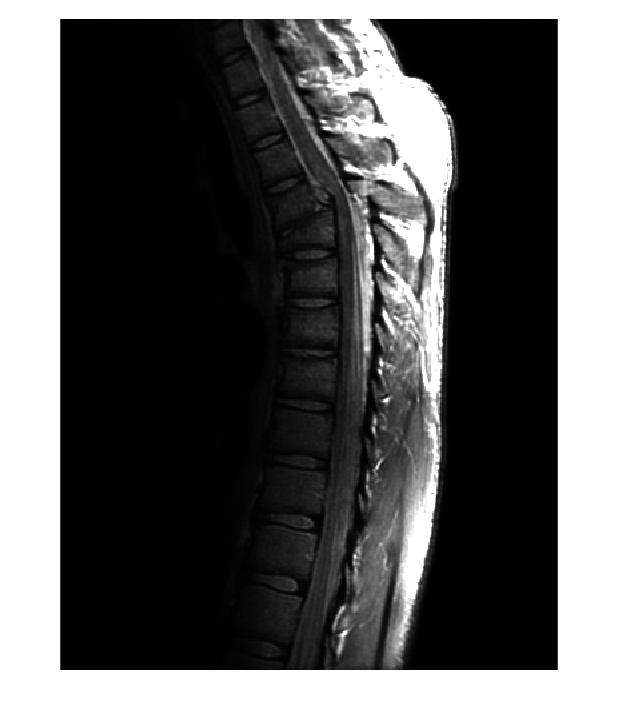
\includegraphics[scale=0.2]{0308}
\caption{Original Image}
\label{fig:original}
\end{figure}
\subsubsection{Log Transformations}
The general form of the log transformation is
$$ s=clog(1 + r) $$
where $r$ is the original pixel value between 0 and 1, $s$ is the pixel value after log transformation and $c$ is a constant. By observing the function we could find that this transformation maps a narrow range of low intensity values in the input into a wider range of output levels. We could use this kind of transformation to expand the values of dark pixels in the given MRI and compressing the higher-level values, which could show the details of the fractured part more obvious. 
\subsubsection{Power-Low(Gamma) Transformations}
Power-law transformations have the basic form
$$ s = cr^{\gamma} $$
Where where $r$ is the original pixel value between 0 and 1 and $s$ is the pixel value after transformation. $c$ and $ \gamma $ are positive constants. By observing the equation we could find that power-law transformation also map a narrow range of dark input values into a wider range of output values. By analyzing, we could notice that when $\gamma > 1$, the produced image tend to be darker than the original image. However, when $\gamma < 1$, the produced image will show more details on dark area of original image. In the following experiments, we need to find appropriate $c$ and $\gamma$ to show more details of the given MRI.
\subsection{Discussion of Results}
\subsubsection{Experiments of Log Transformations}
The experiments results of log transformation shows below:
\begin{figure}[h]
	\centering
	\subfloat[Subfigure 1 list of figures text][Original Image]{
		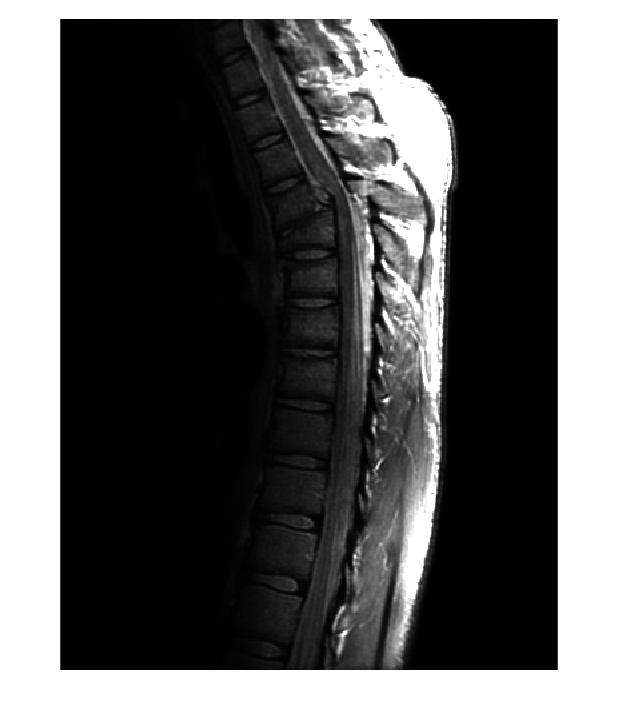
\includegraphics[width=0.2\textwidth]{0308}
		\label{fig:subfig1}}
	\subfloat[Subfigure 2 list of figures text][$c=1$]{
		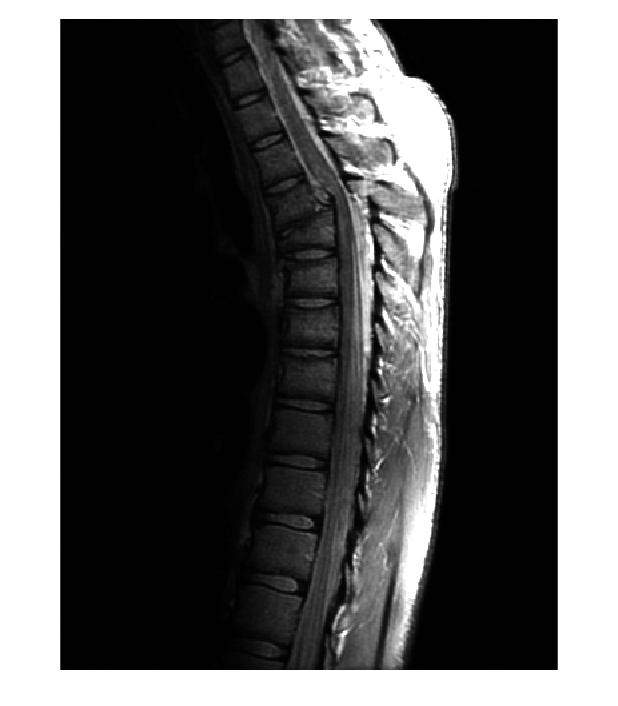
\includegraphics[width=0.2\textwidth]{logc1}
		\label{fig:subfig2}}
	\subfloat[Subfigure 3 list of figures text][$c=3$]{
		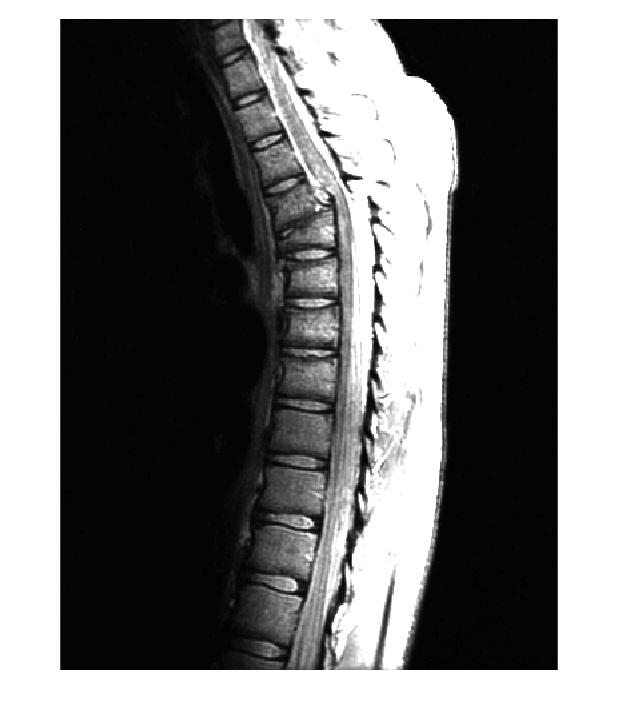
\includegraphics[width=0.2\textwidth]{logc3}
		\label{fig:subfig3}}
	\subfloat[Subfigure 4 list of figures text][$c=6$]{
		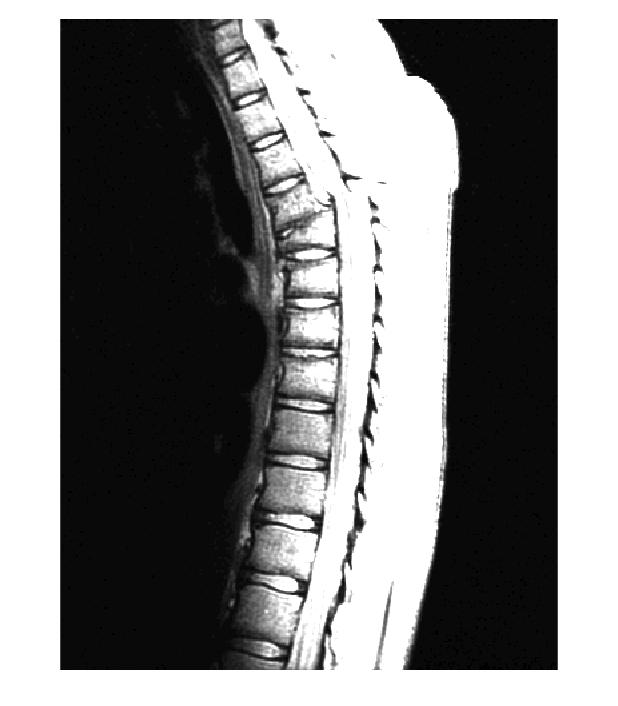
\includegraphics[width=0.2\textwidth]{logc6}
		\label{fig:subfig4}}
	\label{fig:exlogfig}
	\caption{Experiments results of log transformation when $c=$ 1, 3 and 6}
\end{figure}
As shown in Figure \ref{fig:subfig2}, the produced image shows more details on the dark area compare with the given MRI. However, the fractured area on the dark side still not clear enough. When we have $c=6$, we could find even more details on the dark area as it shows in Figure \ref{fig:subfig4}. But we could also notice that those area around the fractured point become totally white, which may result in missing of important information. As shown in Figure \ref{fig:subfig3} When $c=3$, we could have a relative desirable output image since it provides us enough information about the fracture also dark area. 
\begin{figure}[h]
\centering
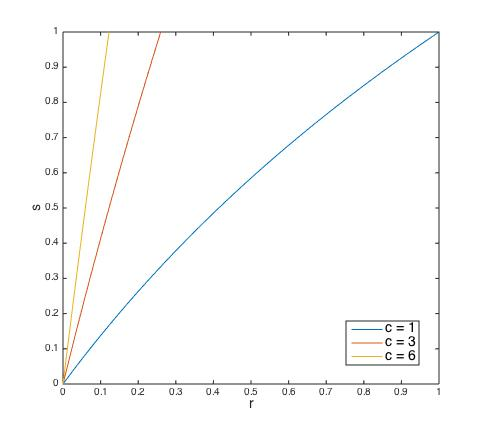
\includegraphics[scale=0.4]{log136}
\caption{The curve of $clog(r + 1)$ when $c =$ 1, 3 and 6}
\label{fig:curvelog}
\end{figure}
The reason behind it could be found in Figure \ref{fig:curvelog}. So, when $c=3$ the output image could have best visual enhancement.
\subsubsection{Experiments of Power-Low Transformations}






\section{Part B}
\subsection{Technical Discussion}
\subsubsection{Histogram Processing}
The histogram of a digital image with intensity levels in the range [$0, L - 1$] is a discrete function $h(r_k) = n_k$, where $r_k$ is the $k$th intensity value and $n_k$ is the number of pixels in the image with intensity $r_k$. It is common practice to normalize a histogram by dividing each of its components by the total number of pixels in the image, denoted by the product $MN$, where, as usual, $M$ and $N$ are the row and column dimensions of the image. Thus, a normalized histogram is given by $p(r_k) = n_k/MN$, for $k = 0, 1, 2, ..., L-1$. Loosely speaking, $p(r_k)$ is an estimate of the probability of occurrence of intensity level $r_k$ in an image. The sum of all components of a normalized histogram is equal to 1.
\subsubsection{Histogram Equalization}
As we know, if we view input intensities $r$ and output intensity $s$ as random variables and their histograms as probability density functions(pdf) $p_r(r)$ and $p_s(s)$.\\
if $p_r(r)$ and $T(r)$ are known and $T(r)$ is continuous and differentiable, then,
$$ p_s(s) = p_r(r)\frac{1}{\left| \frac{ds}{dr} \right|} = p_r(r)\left| \frac{dr}{ds} \right| $$ 
Cumulative distribution function of a random Variable:
$$s = T(r) = (L - 1)\int_0^r p_r(w)dw$$
To fund $p_s(s)$ we have to compute
$$ \frac{ds}{dr} = \frac{dT(r)}{dr} = (L - 1)\frac{d}{dr}\int_0^r p_r(w)dw = (L - 1)p_r(r) $$
Substituting this result:
$$ \frac{ds}{dr} = (L - 1)p_r(r) $$
to 
$$ p_s(s) = p_r(r)\left| \frac{dr}{ds} \right| $$
yields
$$p_s(s) = p_r(r)\left| \frac{1}{(L - 1)p_r(r)} = \frac{1}{L - 1} \right|, 0 \leq s \leq L - 1 $$
The formula for histogram equalisation in the discrete case is given
$$ s_k = T(r_k) = (L - 1)\sum_{j = 0}^k p_r(r_j) = \frac{L - 1}{MN}\sum_{j = 0}^{k} n_j $$
\subsection{Discussion of Results}
\subsubsection{Computing the histogram of an image}
The original image is shown in Figure \ref{fig:hisoriginal}
\begin{figure}[h]
	\centering
	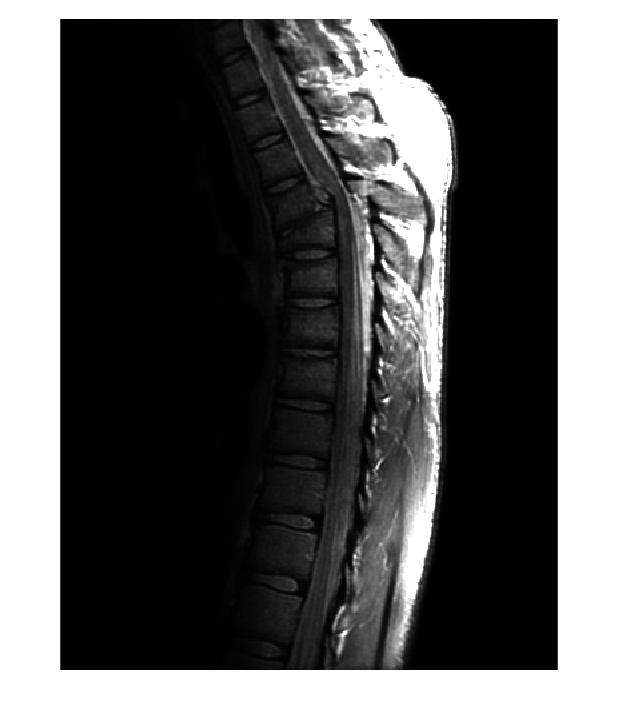
\includegraphics[scale=0.2]{0308}
	\caption{Original Image}
	\label{fig:hisoriginal}
\end{figure}
To get the histogram of given image, we need to iterate all pixel values of the image and get the frequency of each intencity. Figure \ref{fig:hishist1} shows the output histogram of Figure \ref{fig:hisoriginal} after normalisation. We can note that most pixel values are on the dark side.
\begin{figure}[h]
	\centering
	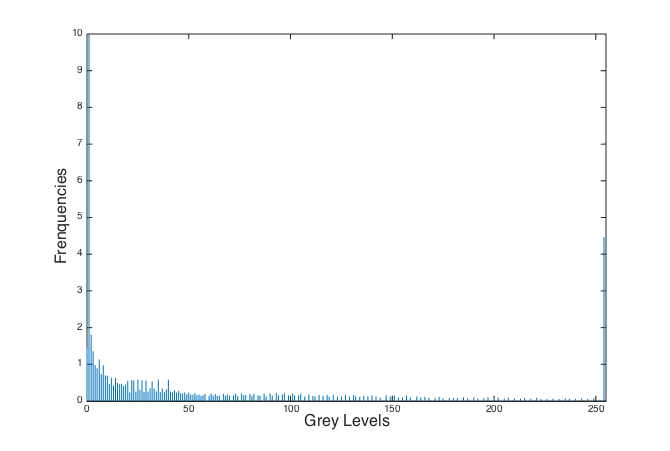
\includegraphics[scale=0.4]{historg}
	\caption{Histogram of Figure \ref{fig:hisoriginal}}
	\label{fig:hishist1}
\end{figure}
\subsubsection{Implemention of histogram equalization}
To perform histogram equalization on given image, we could use the formula for histogram equalization in the discrete case
$$ s_k = T(r_k) = \frac{L - 1}{MN}\sum_{j = 0}^{k} n_j $$
\\[10cm]
\begin{figure}[h]
	\centering
	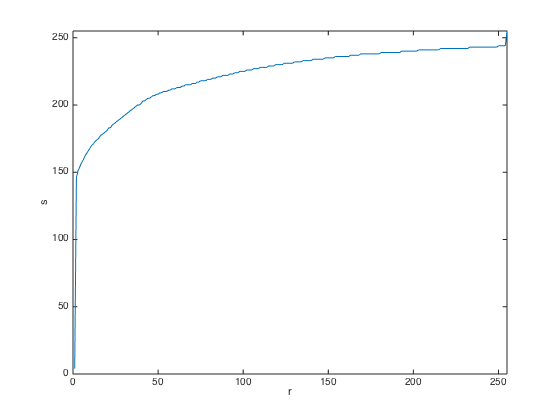
\includegraphics[scale=0.4]{hetrans}
	\caption{Transformation function}
	\label{fig:hetrans}
\end{figure}

Figure \ref{fig:hetrans} shows the transformation function. Figure \ref{fig:histeq} shows the comparision between the original image and the image after histogram equalization. We can notice that the produced image is much lighter than original image and we could get more details on the darker side of the image. However, the background became too light after histogram equalization, which reduce the contrast of image. Figure \ref{fig:histnew} shows the histogram of the produced image. \\
\\
The reason of the background became too light can be described as follows. As we can see from the histogram of original image in Figure \ref{fig:hishist1}, most of the pixel values in orinal image are concentrated neat 0. According to the formula for histogram equalization in the discrete case
$ s_k = T(r_k) = \frac{L - 1}{MN}\sum_{j = 0}^{k} n_j $, if there are too many pixel values nears 0, then the output value $s$ will grow a lot for those input pixels with value near 0. As a result, the produced image have a washed-out appearance. 
\begin{figure}[h]
	\centering
	\subfloat[Subfigure 1 list of figures text][Original Image]{
		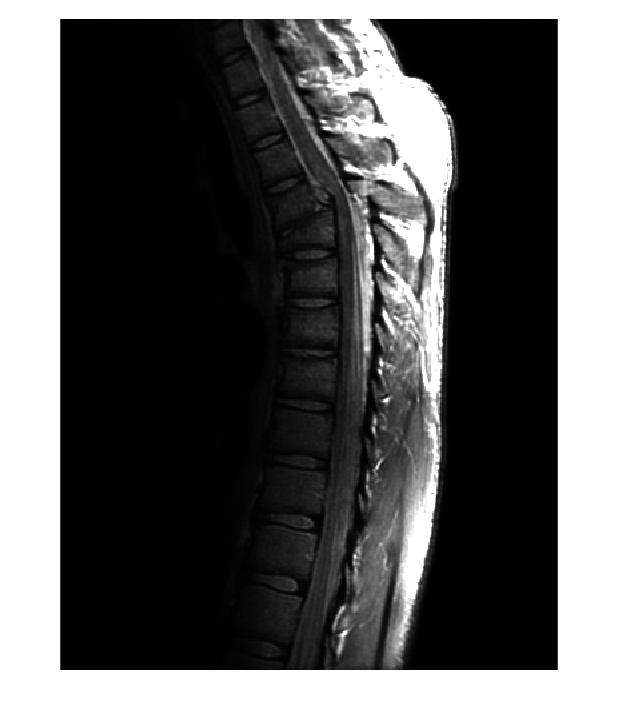
\includegraphics[width=0.2\textwidth]{0308}
		\label{fig:histeqsub1}}
	\subfloat[Subfigure 2 list of figures text][Image after histogram equalization]{
		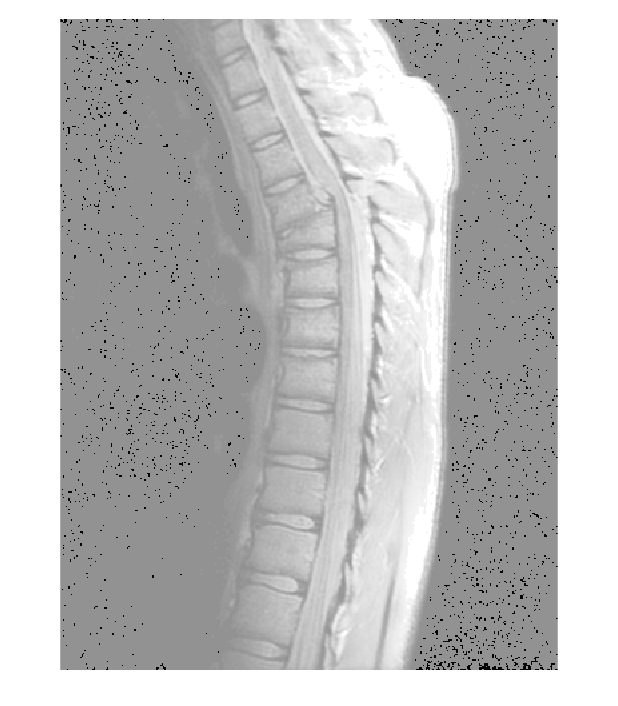
\includegraphics[width=0.2\textwidth]{histeq}
		\label{fig:histeqsub2}}
	\caption{Experiments results of histogram equalization}
	\label{fig:histeq}
\end{figure}

\begin{figure}[h]
	\centering
	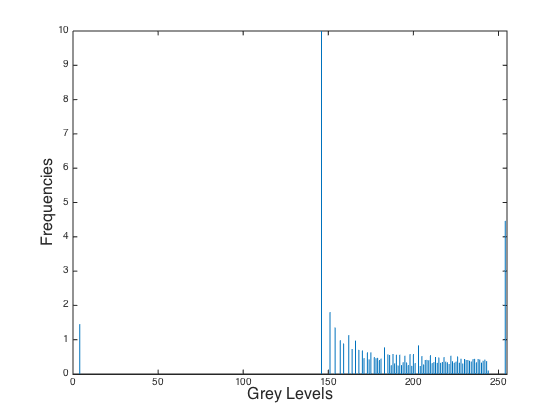
\includegraphics[scale=0.4]{histnew}
	\caption{Histogram of produced image}
	\label{fig:histnew}
\end{figure}
\newpage
\section{Appendix}
\subsection{Program of Log Transformation}
\begin{lstlisting}
%*****************
%Student Name: Yang Wang
%Student #: 1001319227
%Title: Log Transformation
%*****************
clear;
clc;
cla;
c = 3;
G = imread('0308.tif');
[rows, cols] = size(G);
for i = 1 : rows
    for j = 1 : cols
       G(i, j) = c * log2(double(G(i, j))/255.0 + 1) * 255.0;
    end
end 
figure();
imshow(G);    
\end{lstlisting}

\subsection{Power-Law Transformation}
\begin{lstlisting}
%*****************
%Student Name: Yang Wang
%Student #: 1001319227
%Title: Log Transformation
%*****************
clear;
clc;
cla;
c = 1;
gamma = 0.4;
G = imread('0308.tif');
[rows, cols] = size(G);
for i = 1 : rows 
    for j = 1 : cols
        G(i, j) = c * 255 * (double(G(i, j))/255)^gamma;
    end
end
figure(2);
imshow(G);   
\end{lstlisting}

\subsection{Program of computing histogram}
\begin{lstlisting}
%*****************
%Student Name: Yang Wang
%Student #: 1001319227
%Title: Computing Histogram of image
%*****************

clear;
clc;
cla;
G = imread('0308.tif');
H = zeros(1, 256);
[rows, cols] = size(G);
for i = 1 : rows
    for j = 1 : cols
       H(1, G(i, j) + 1) = H(1, G(i, j) + 1) + 1;
    end
end
%show histogram of image after normalization
x = 0 : 255;
figure(1)
H = H * 100 / (rows * cols);
stem = stem(x, H);
set(stem, 'Marker', 'none');
axis([0 255 0 10]);
\end{lstlisting}

\subsection{Program of histogram equalization}
\begin{lstlisting}
%*****************
%Student Name: Yang Wang
%Student #: 1001319227
%Title: Histogram Equalization
%*****************

clear;
clc;
cla;
G = imread('0308.tif');
H = zeros(1, 256);
[rows, cols] = size(G);
for i = 1 : rows
    for j = 1 : cols
       H(1, G(i, j) + 1) = H(1, G(i, j) + 1) + 1;
    end
end
nums = rows * cols - 1;
collects = zeros(1, 256);
for i = 1 : 256
    if(i == 1) 
        collects(i) = (double(H(i)) / nums) * 255;
    else
        collects(i) = (double(H(i)) / nums) * 255 + collects(i - 1);
    end
end
k = uint8(collects);
for i = 1 : rows
    for j = 1 : cols
       G(i, j) = k(1, G(i, j) + 1);
    end
end
%show image after HE
figure(1);
imshow(G);
x = 1 : 256;

%transformation function
figure(2);
s2 = plot(x, k);
xlabel('r');
ylabel('s');
axis([0 255 0 255]);

%histogram after HE
H = zeros(1, 256);
[rows, cols] = size(G);
for i = 1 : rows
    for j = 1 : cols
       H(1, G(i, j) + 1) = H(1, G(i, j) + 1) + 1;
    end
end
x = 0 : 255;

figure(3)
H = H * 100 / (rows * cols);
stem = stem(x, H);
set(stem, 'Marker', 'none');
axis([0 255 0 10]);
\end{lstlisting}


\end{document}